\chapter{Integration Notes}

\section{Integration into a Project}
\ifnum \DocumentGroup=1{
Please refer to the installation instructions included in the RTA-SUM Getting Started Guide to generate the RTA-SUM SOH directly inside
ISOLAR-AB. Briefly you can select RTA Code Generator for configuring the SUM Modules that want to be integrated in the project accordigly
to its Model Year (MY) version. When the option "Not Configured" is selected, the module will not be integrated.
}
\else{
There is no need for standard installation procedure for SOH. The folder itself contains all the necessary
artifacts to integrate into a project. Dropping the complete folder structure into a BSW configuration
project will enable the user to configure SOH and generate all the necessary artifacts.
}
\fi

Refer to \href {https://rtahotline.etas.com/confluence/display/RH/RTA-SUM} {RTA-SUM Knowledge Base}

\section{Module Dependencies}
When connecting the Dcm to the port interface \code{DataServices<SOH>Data<n>} the DID counters\newline \code{DID 0xF08F, DID 0xF090, DID 0xF091, DID 0xF092, DID 0xF093} will be updated through operation invoked event Runnables.\\
\\
If OS Status Monitoring is enabled (look \ref{subsection:sohGeneral}), please Make reference to  \ref{section:configOS}.

\section{Configuring SOH}
Once the complete package has been added to a BSW project, an additional module SOH should
appear. From here you can open and begin configuring the module. Specific description of each
configurable parameter is available in the “Description” view of \ifnum \DocumentGroup=1{ISOLAR-AB}\else{ISOLAR-A with BCT add-on}\fi \hfill
when a parameter is selected.

\section{Generating Artifacts}
Generating the C/H/SWCD files from your configuration is similar to other BSW modules delivered
from ETAS. The Code Generation perspective of the \ifnum \DocumentGroup=1{ISOLAR-AB}\else{ISOLAR-A with BCT add-on}\fi, will present the user with a dialog
to select specific module within the project to generate.\ifnum \DocumentGroup=1{}\else{Either a Partial Build or Full Build can be used, depending on the needs of the user.}\fi In case of any configuration errors present in SOH, the
console window will output a description of any errors found during generation. Further, when the
user is configuring the module, the Problems Log will show any active errors in the configuration of
SOH. A third visual aid is the appearance of red X’s in the configuration view over items which are invalid. 
Simply hovering over these X’s will provide the user a description of the problem. These are static validations.

\section{Configuring the RTE}
\label{sec:rte}
After the user has configured and generated the artifacts for SOH, the output SWCD file\newline
(SUM\_SOH\_Swcd.arxml) can be used for the RTE configuration. This is a complete SWC description
per the AUTOSAR standard of all the users configured ports and interfaces required for the project
specific configuration. This SWCD is a standard ASW component and not a module description. Therefore,
there are no special considerations to be taken into account when configuring the RTE. It is
recommended that if specific changes are required to the SWCD, the user not manually edit this file,
rather update and regenerate the configuration with the required changes.


The minimum \textbf{RTA-RTE version} supported is the \textit{7.3.0}.


Note: RTE command used for RTE generation

\begin{rtecommandline}
-err=xml -nts --samples=memmap --os-define-osenv=RTAOS40 --exclusive-area-optimization=disable --os-output-param=all --strict-unconnected-rport-check=off
\end{rtecommandline}

\section{Configuring OS}
\label{section:configOS}
The following integration notes about the OS configuration consider RTA-OS version 6.0.0 by ETAS for reporting examples, templates and Samples but it can be adopted for each RTOS.
\\
SUM\_SOH module shall monitor the OS Errors occurrences. This implicates that SUM\_SOH has got a way to be notified by OS about the OS Error Occurrence.
The notification between OS and SUM\_SOH is possible thanks the following Callbacks functions:

\begin{itemize}
    \item \code{ErrorHook}
	\item \code{ProtectionHook}
    \item \code{SOH_OS_Protection_ErrorHook_CallBack}: look \ref{subsubsection:msrm}
\end{itemize}

The \code{ErrorHook} and \code{ProtectionHook} Callbacks are customized functions and \textbf{are in the responsibility of the Integrator/User, according to its OS specification};\newline

ErrorHook/ProtectionHook Callbacks shall be called by OS each time that one of its API produces an Error, in order to identify the type of OS Error and handle it for ensuring the right System Running.\newline

To notify the SUM\_SOH about the OS Error Occurrence it is necessary to call function \newline \code{SOH_OS_Protection_ErrorHook_CallBack} within the ErrorHook and ProtectionHook, passing the ErrorType as function parameter to them.
Figure \ref{fig:errorHook} shows the intended sequences to report an OS Error to SUM\_SOH.

\begin{figure}[h!]
	\centering
	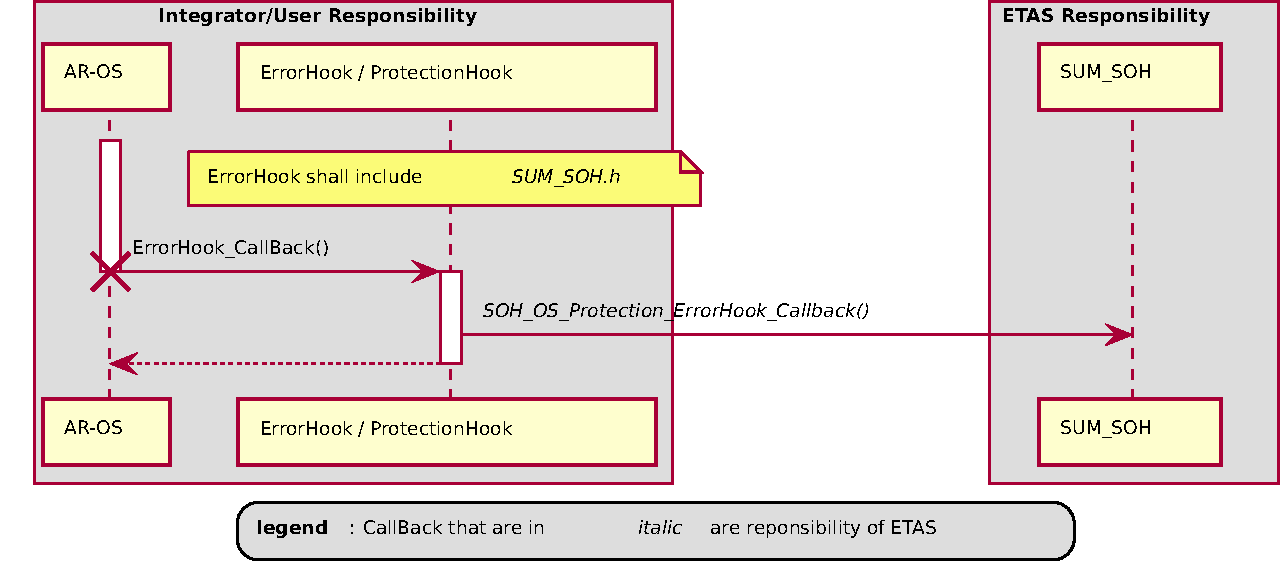
\includegraphics[scale=0.72]{generated/diagrams/errorHook.pdf}
	\caption{Callback sequence to report OS Error to SUM\_SOH}
	\label{fig:errorHook}
\end{figure}

\subsection{OsCounter}
\label{subsec:configOSCounter}
In order to let the Main and Time Manager works properly, the OS Counter shall be configured as follows:		

\begin{itemize}
    \item \code{OsCounterMaxAllowedValue}: The max value that integrator can set is 4294967295 since the tick in the SOH are stored in a uint32;
	\item \code{OsSecondsPerTick}: Choose a value that can provide a good granularity w.r.t. the periodicity of the Runnable Runnable\_SOH\_Timing (configured in SOHGeneral/SOH\_RunnnableSOHTimingPeriod);
\end{itemize}

An example of configuration is provided below: 
\begin{figure}[h!]
	\centering
	\includegraphics[scale=0.9]{images/SOH\_OS\_Counter.png}
	\caption{Example of OsCounter configuration needed.}
\end{figure}

The OsCounter configured SHALL be referenced in the SOHGeneral/Sum\_SOH\_Os\_Counter\_Ref as follow: 

\begin{figure}[h!]
	\centering
	\includegraphics[scale=0.9]{images/SOH\_Counter\_Ref.png}
	\caption{Reference to the OsCounter configured.}
\end{figure}

Please, take into account that the integrator can reference the timer referenced in the SSFM module, parameter Sum\_Ssfm\_Os\_Counter\_1ms\_ref (in Sum\_Ssfm\_General container.)